\documentclass[presentation]{beamer}

\usepackage{appendixnumberbeamer}
\usepackage{amsmath}
\date{18th July 2017}
\usetheme{firedrake}

\author{Lawrence Mitchell\inst{1}}
\institute{\inst{1}Departments of Computing and Mathematics, Imperial College London}
\title{z-layers, oh noes}

\graphicspath{{./\jobname.figures/}}

\newcommand{\arxivlink}[2]{%
  \href{http://www.arxiv.org/abs/#1}%
  {{\small\texttt{arXiv:\,#1\,[#2]}}}%
}
\usepackage{minted}

\begin{document}

\maketitle

\begin{frame}[plain]
  \begin{columns}
    \begin{column}{\textwidth}
      \only<1>{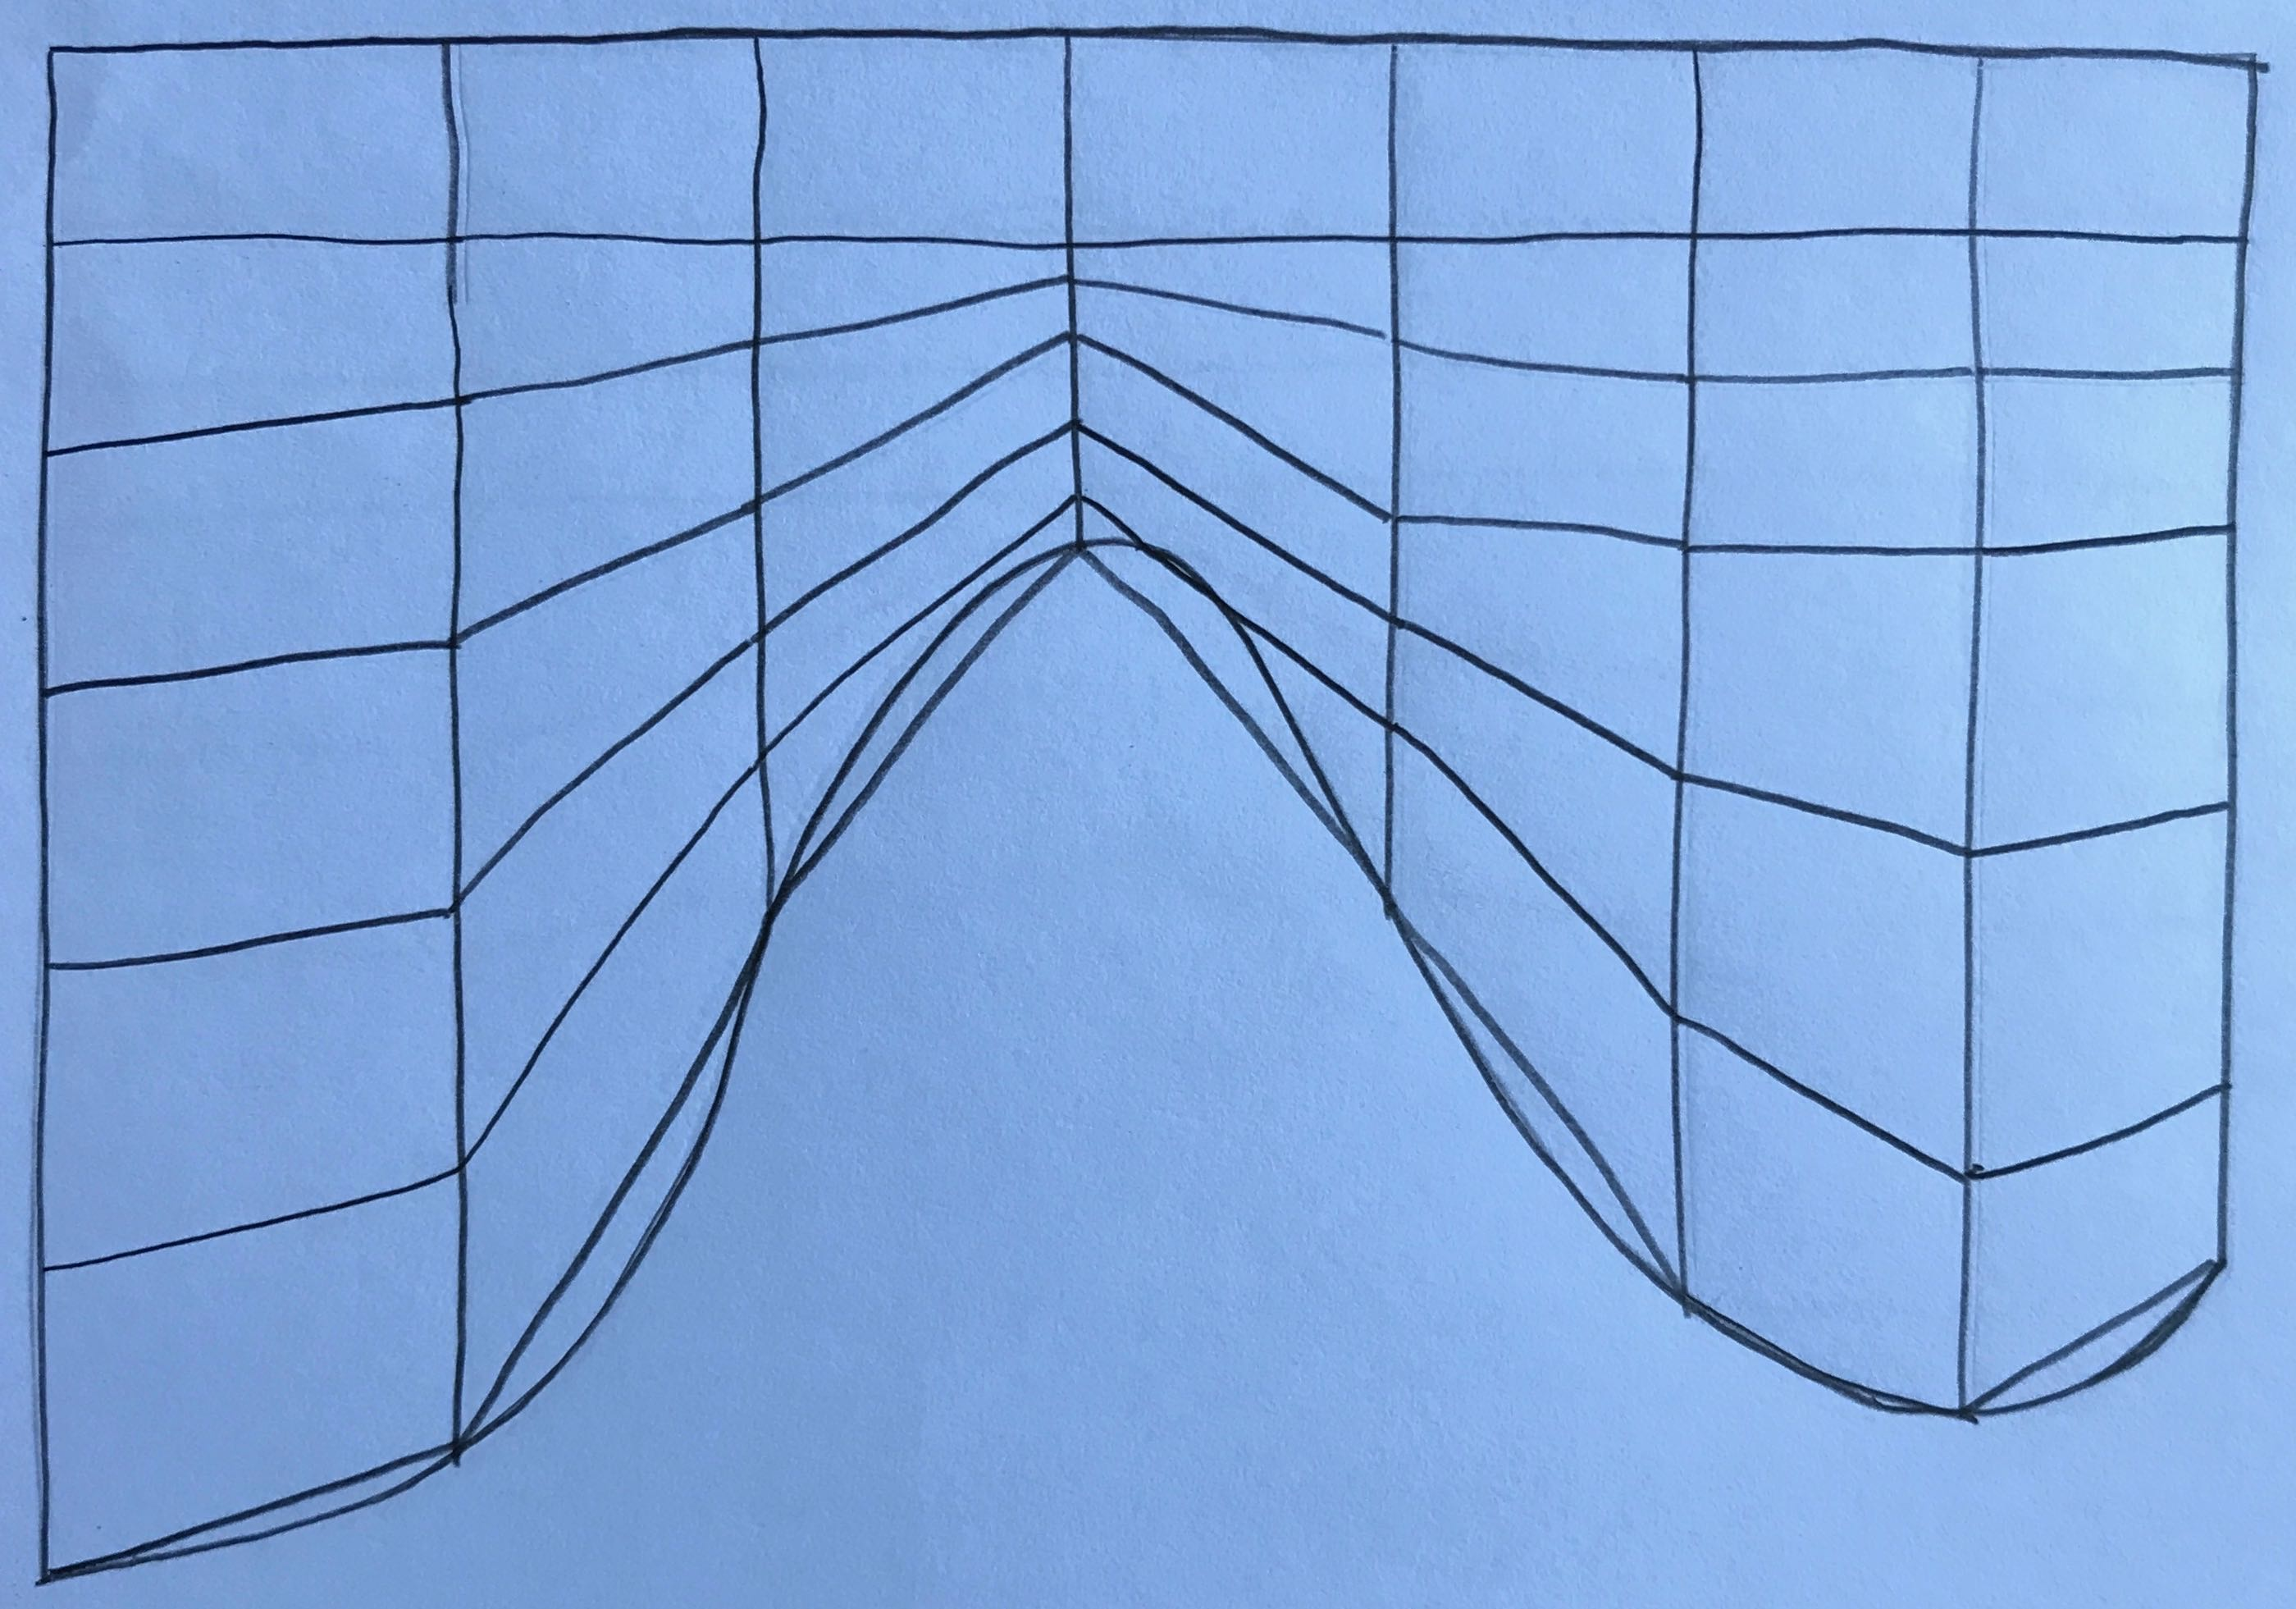
\includegraphics[width=\textwidth]{mountain-sigma}}
      \only<2>{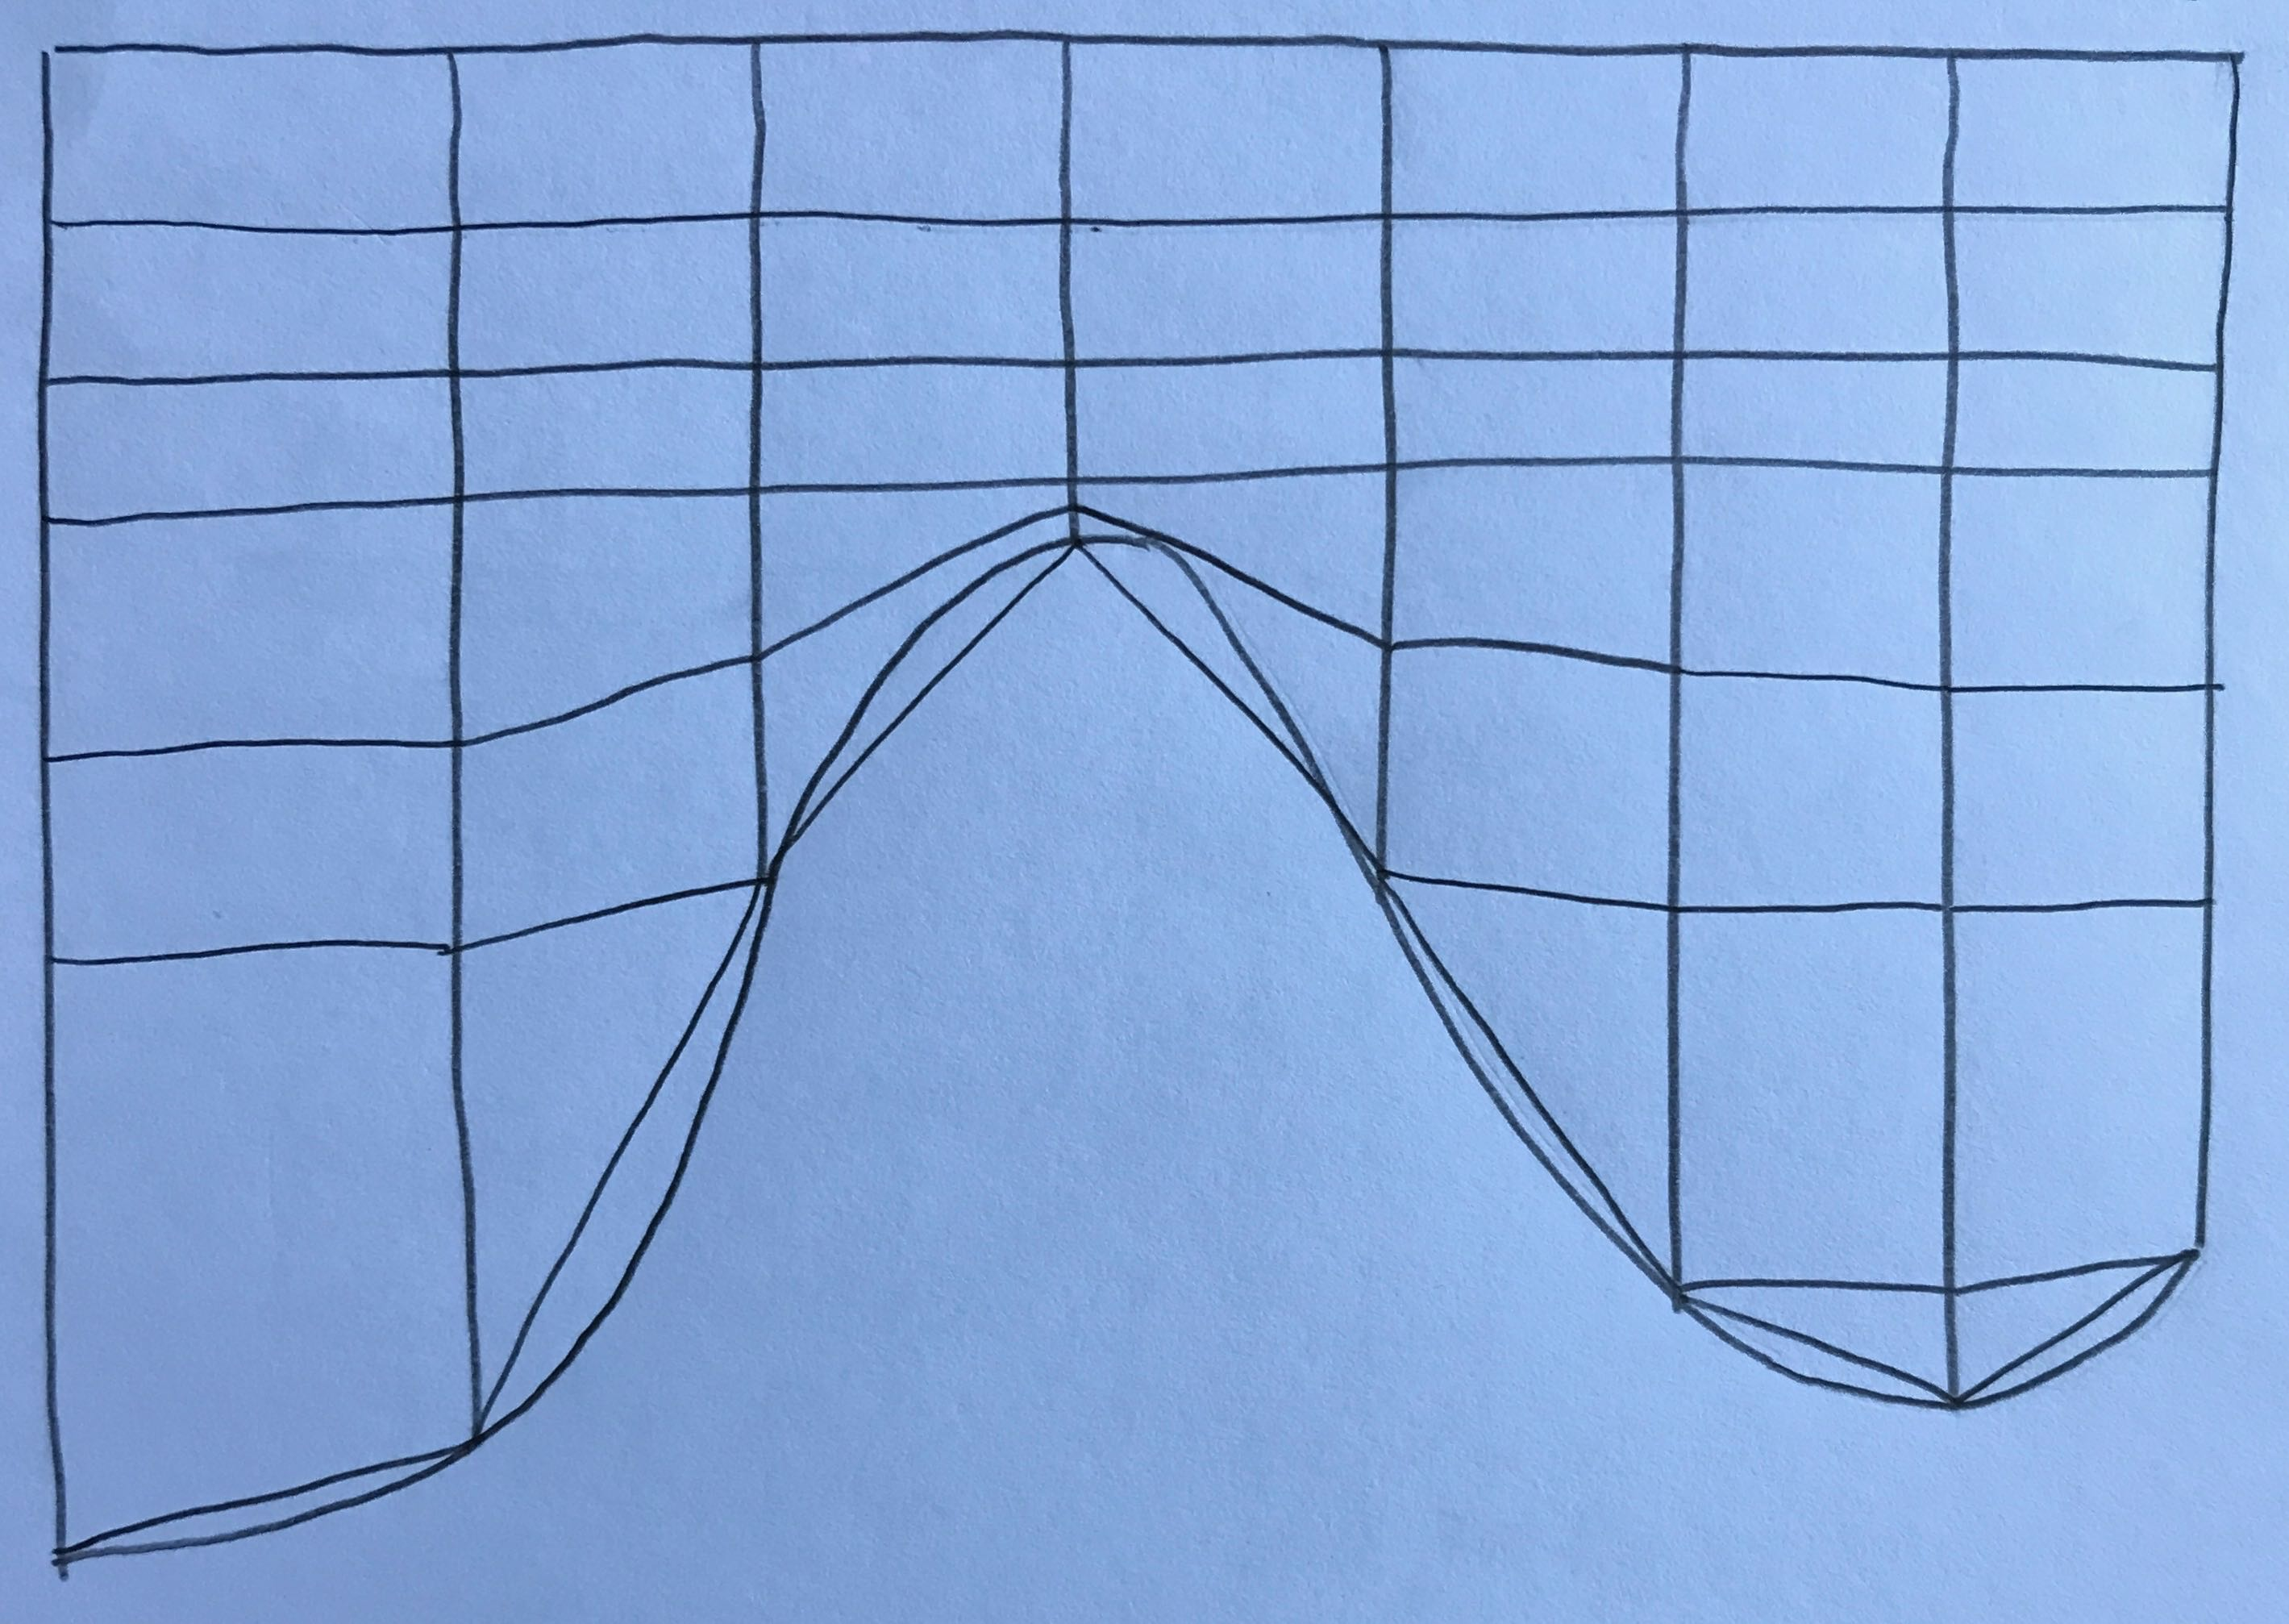
\includegraphics[width=\textwidth]{mountain-z}}
    \end{column}
  \end{columns}
\end{frame}

\begin{frame}
  \frametitle{z-layers}

  \begin{itemize}
  \item Around steep topography, might want to use z-layers rather
    than $\sigma$ coordinates.

  \item Mostly the core computational aspects remain unchanged.

  \item But, the layer number is now \emph{entity}-dependent.

  \item So there's loads more book-keeping.
  \end{itemize}
\end{frame}

\begin{frame}[plain]
  \begin{columns}
    \begin{column}{\textwidth}
      \begin{center}
        \only<1>{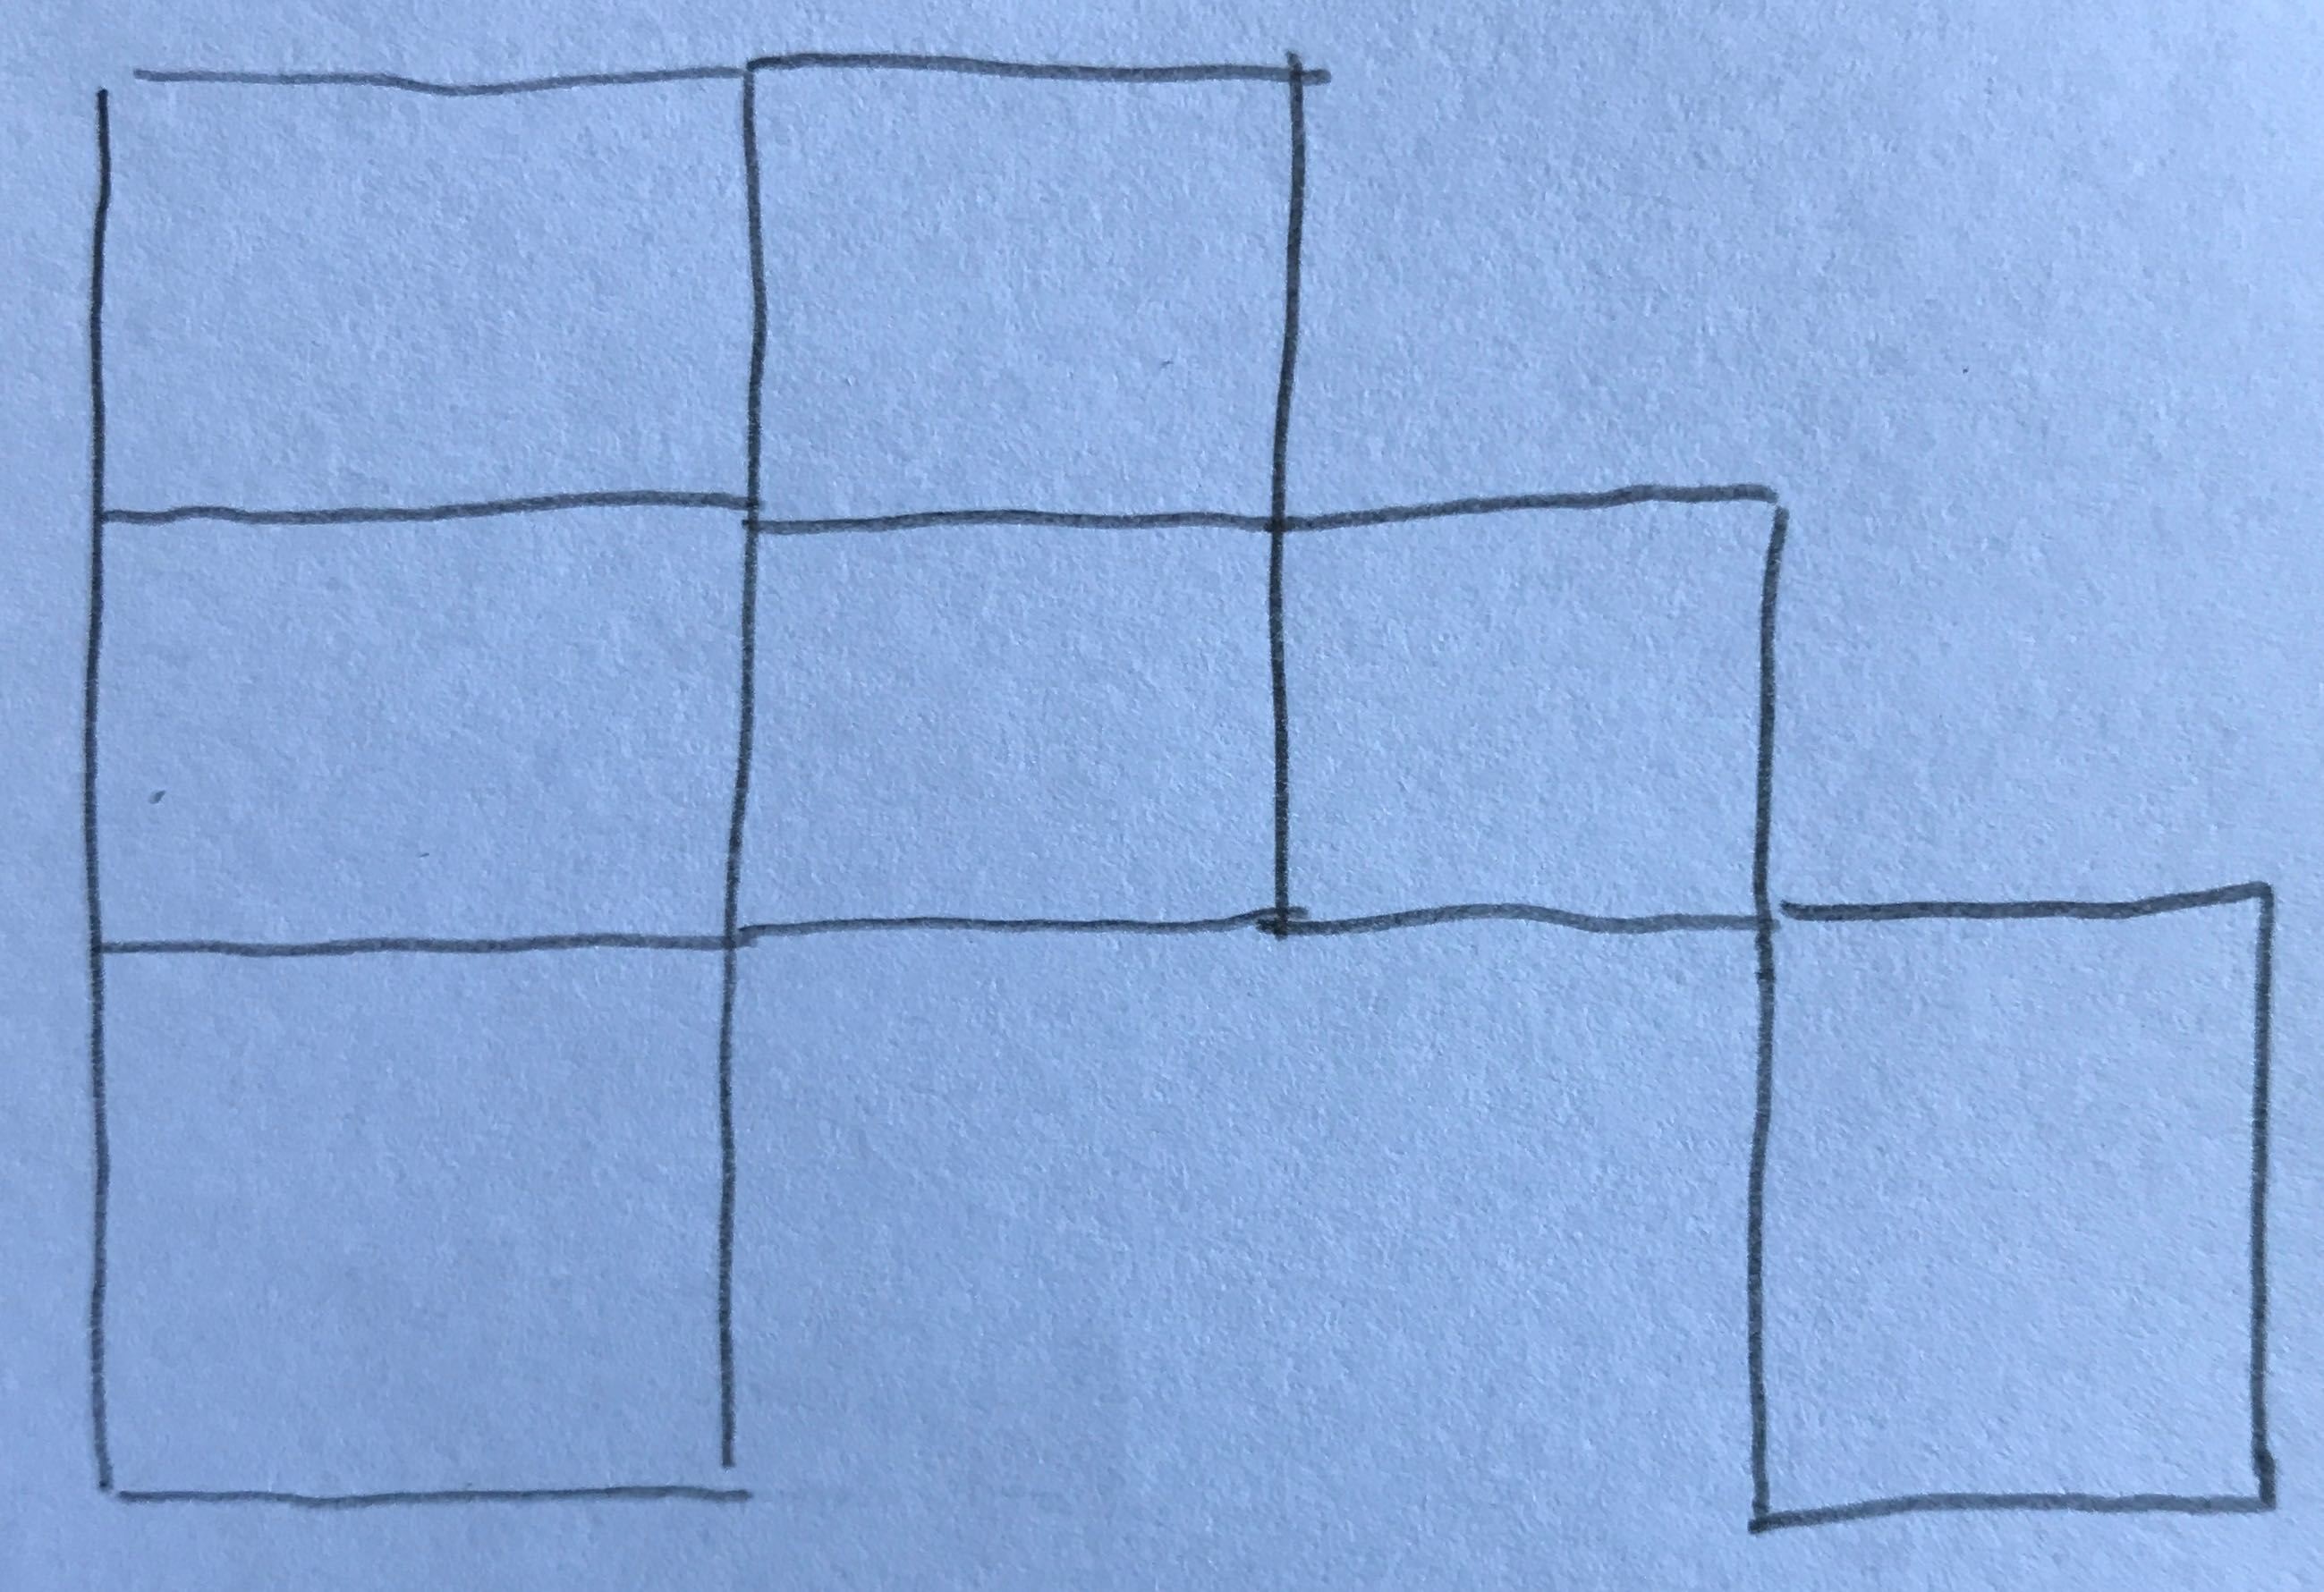
\includegraphics[width=0.9\textwidth]{topology-2d}}
        \only<2>{Provide number of cell layers per base cell

          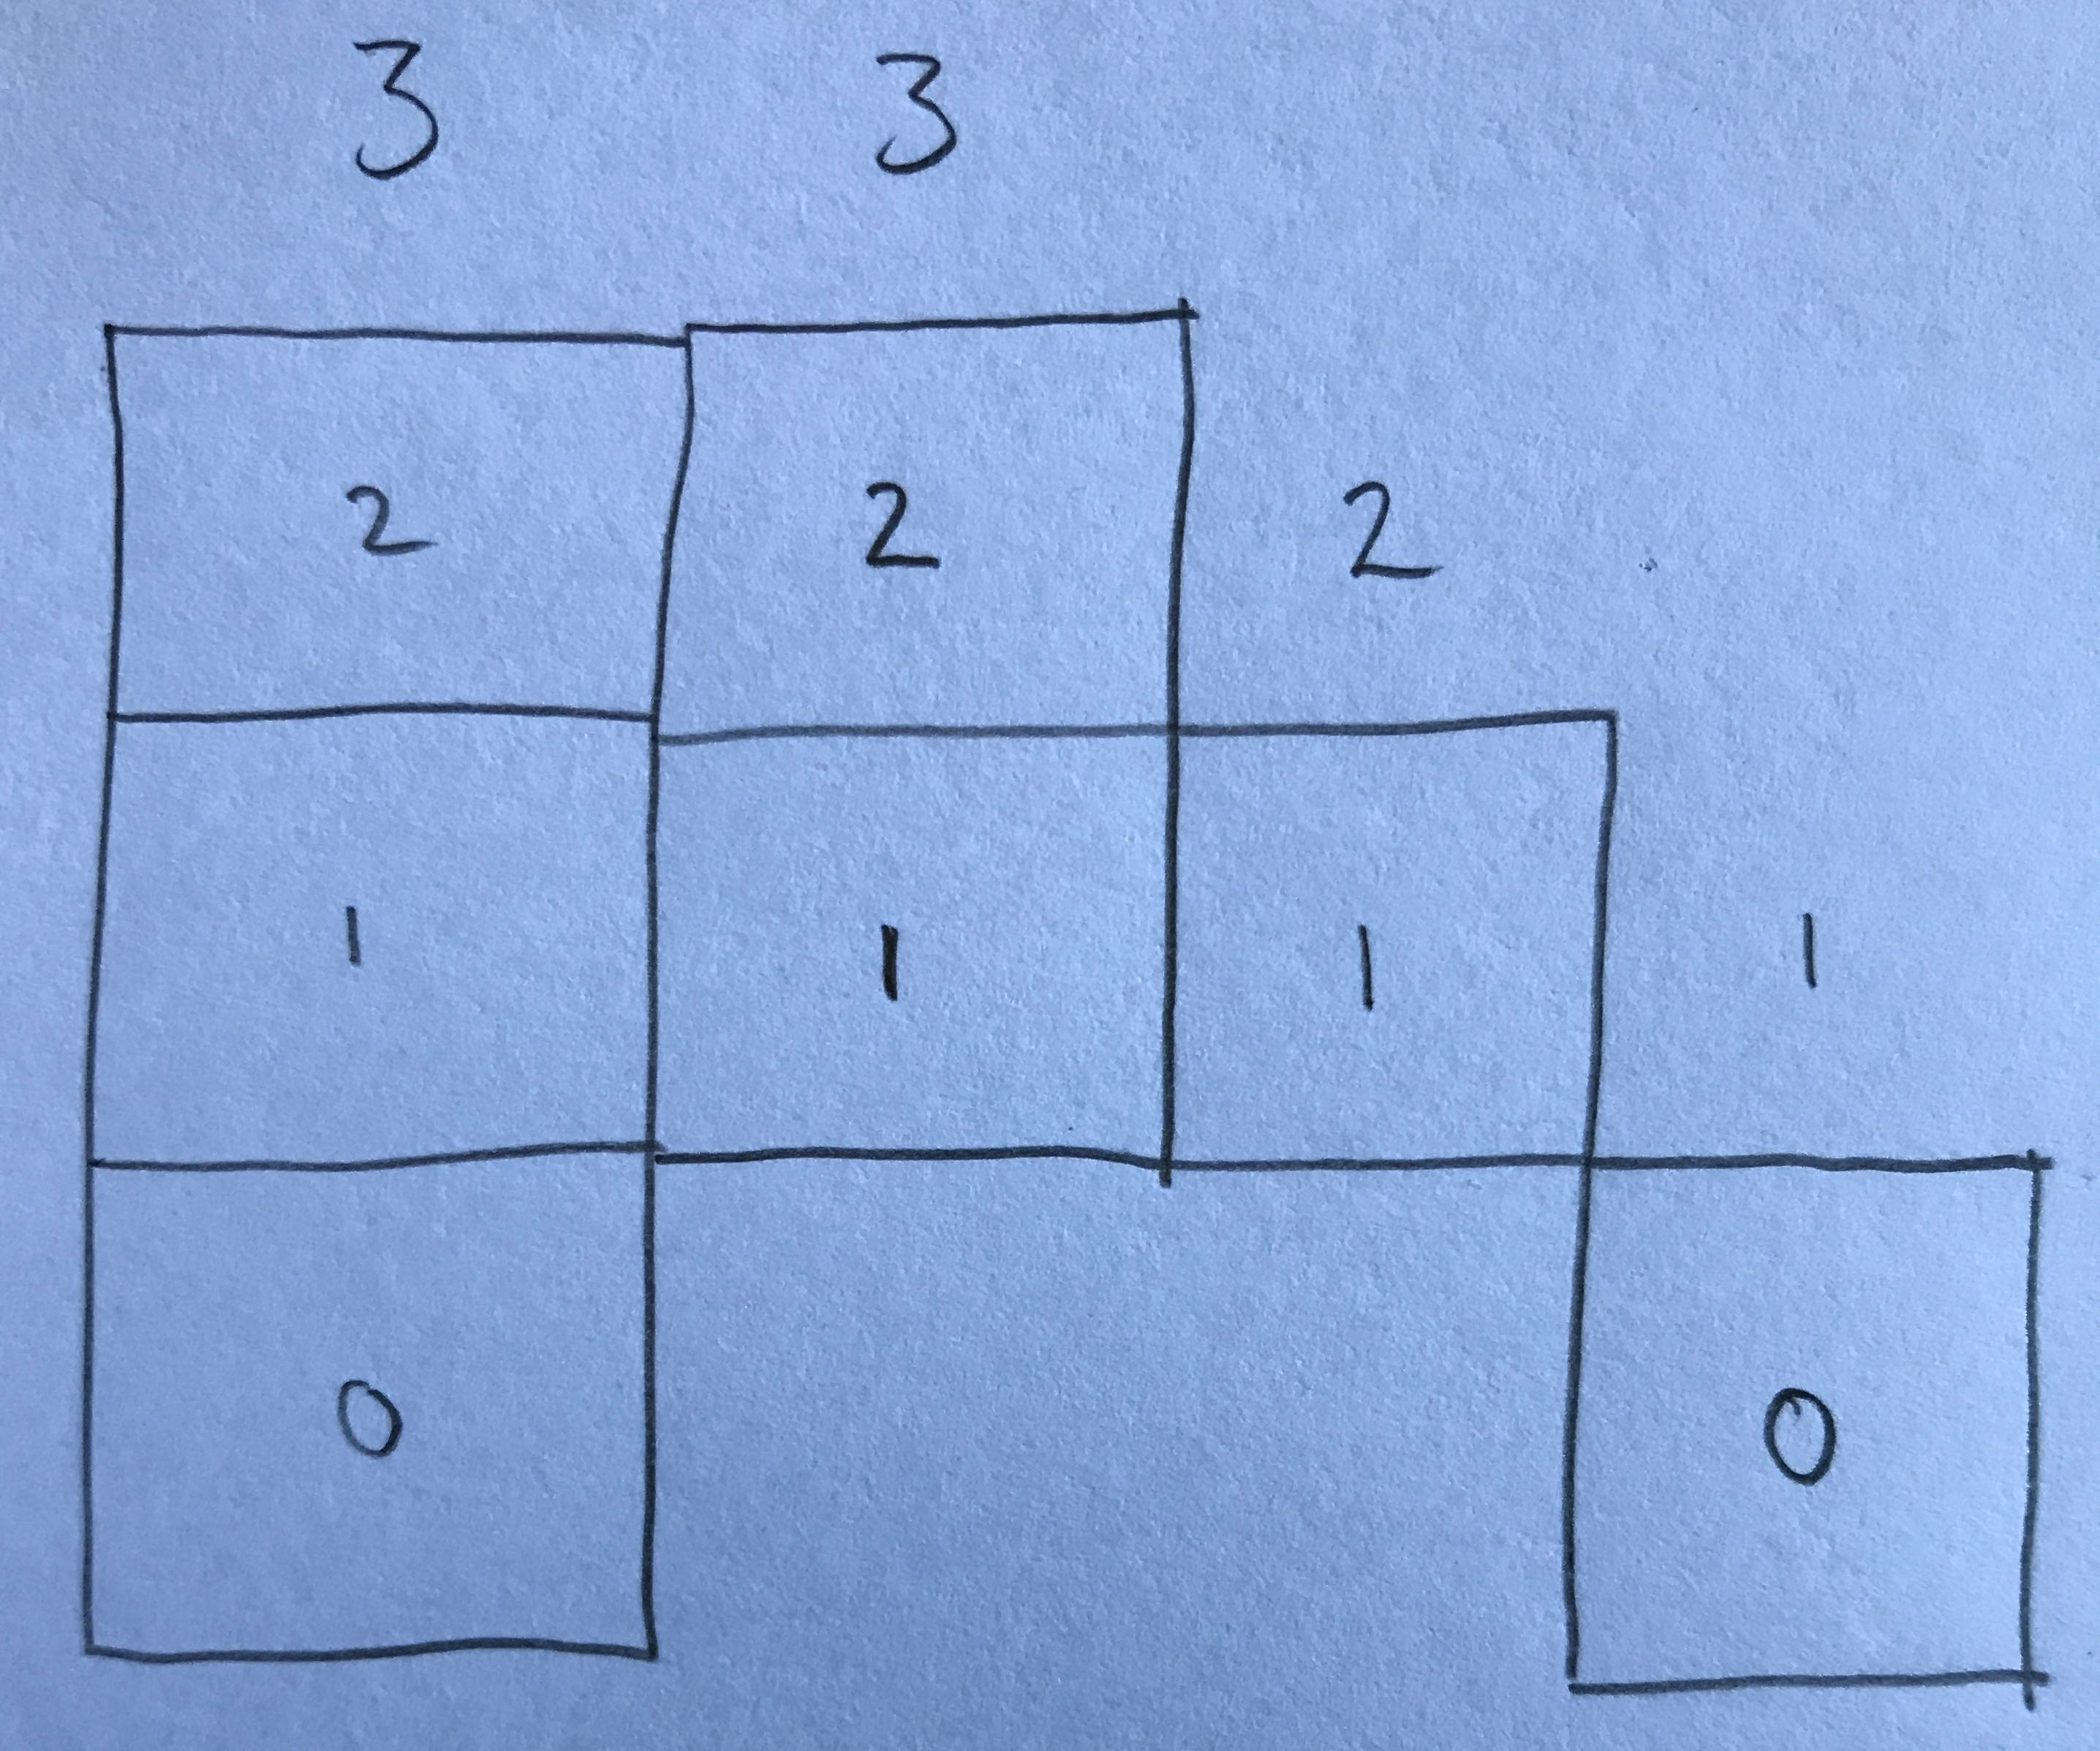
\includegraphics[width=0.8\textwidth]{topology-2d-cells}}
        \only<3>{Bootstrap layers for other entities

          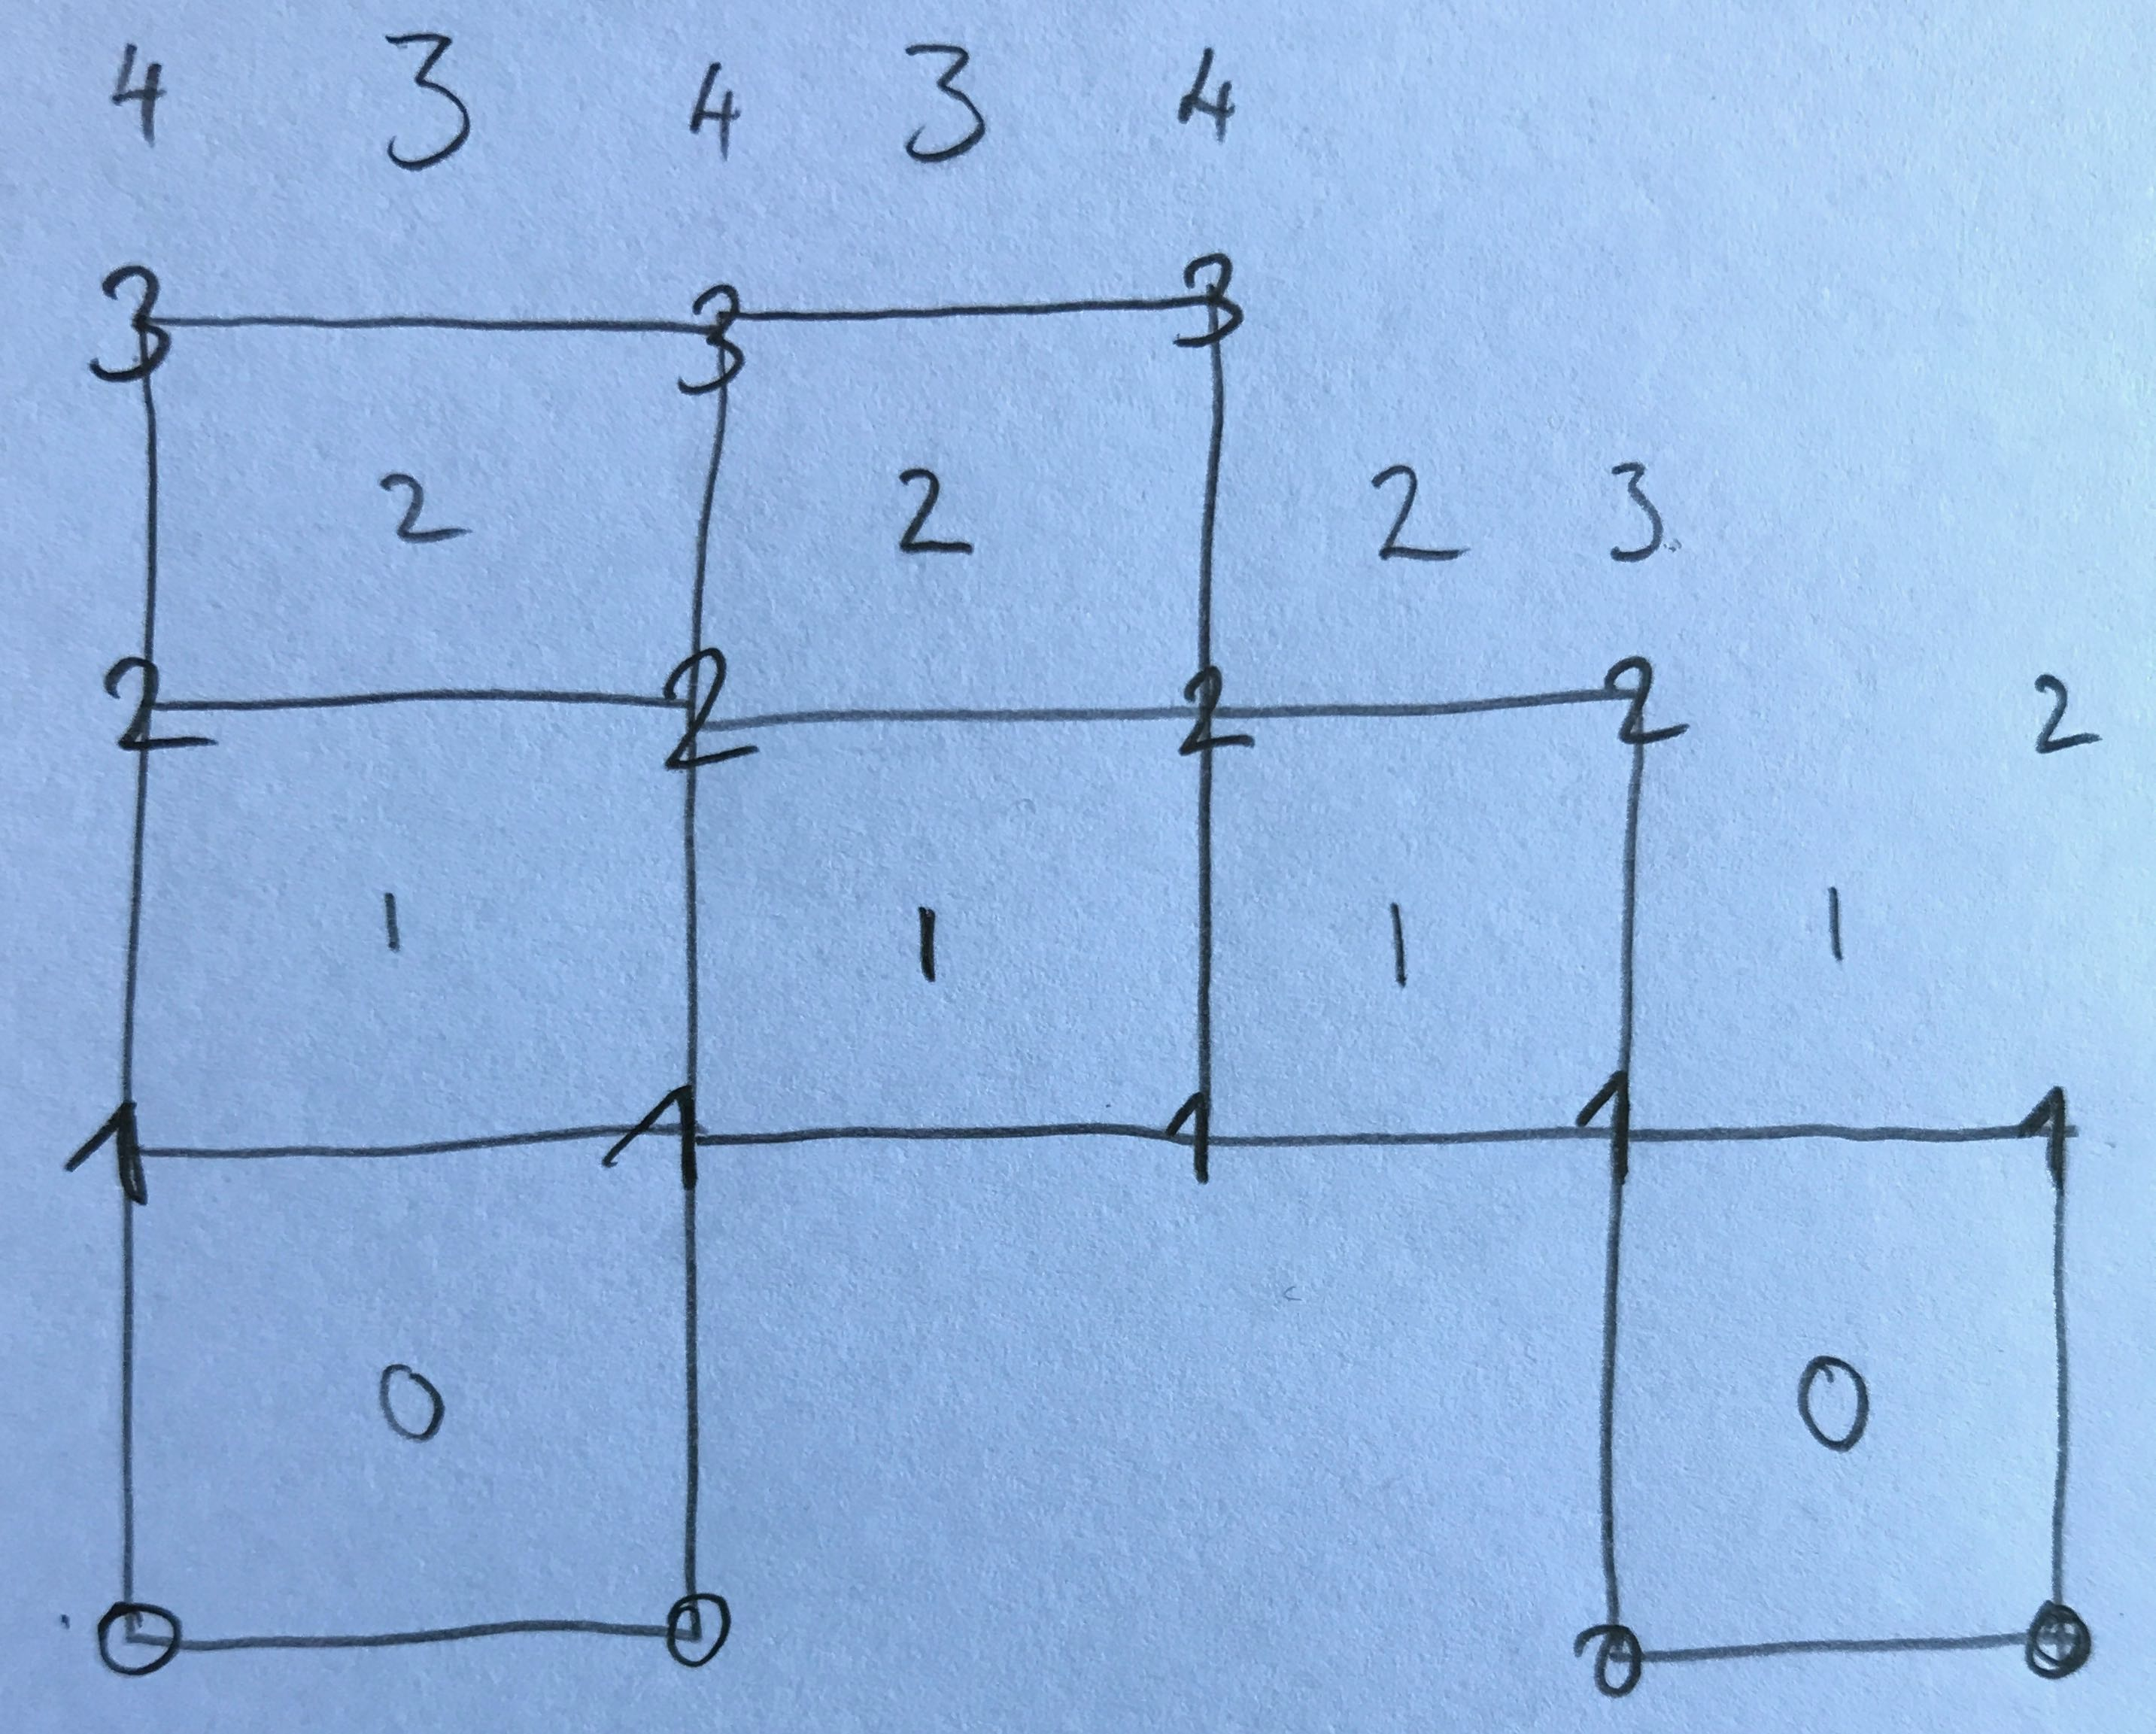
\includegraphics[width=0.8\textwidth]{topology-2d-vertices}}
        \only<4>{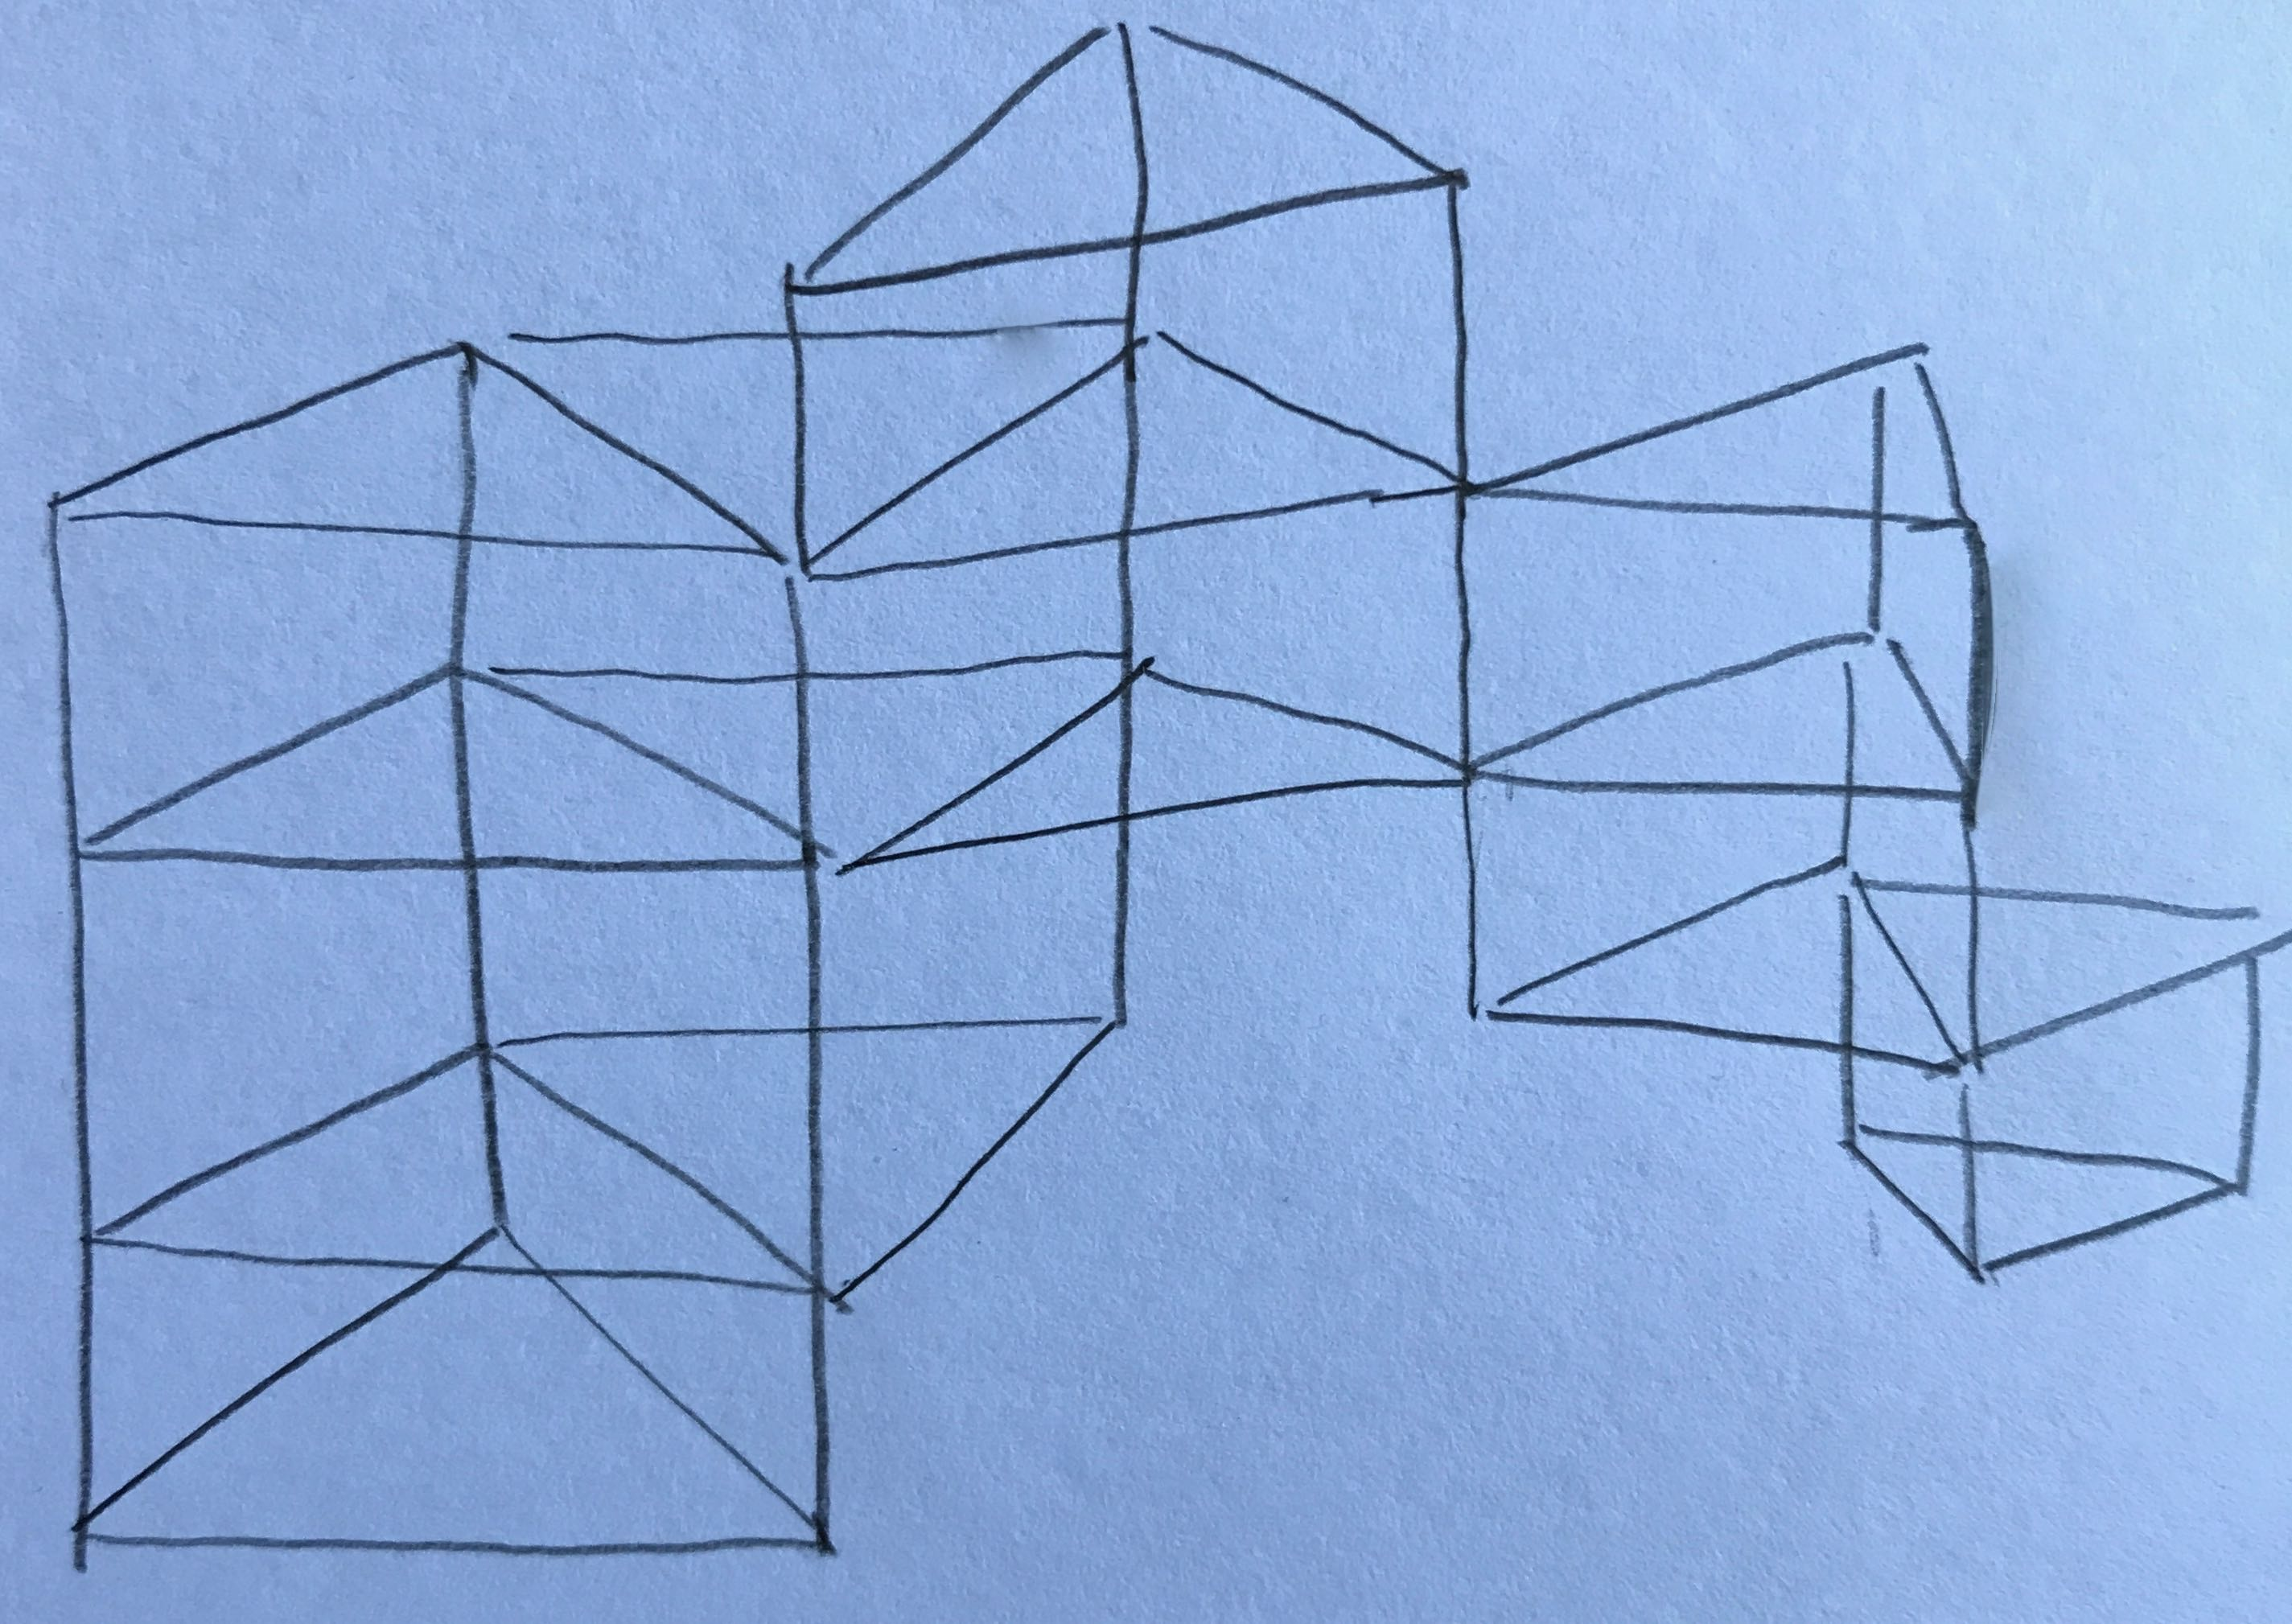
\includegraphics[width=0.9\textwidth]{topology-3d}}
      \end{center}
    \end{column}
  \end{columns}
\end{frame}

\begin{frame}[fragile]
  \frametitle{Mesh construction}
  \begin{itemize}
  \item On each base cell, provide:
    \begin{enumerate}
    \item Start layer (bottom is zero)
    \item Number of cells
    \end{enumerate}
  \end{itemize}
  \begin{columns}
    \hspace{-2em}
    \begin{column}{0.5\textwidth}
      \begin{center}
        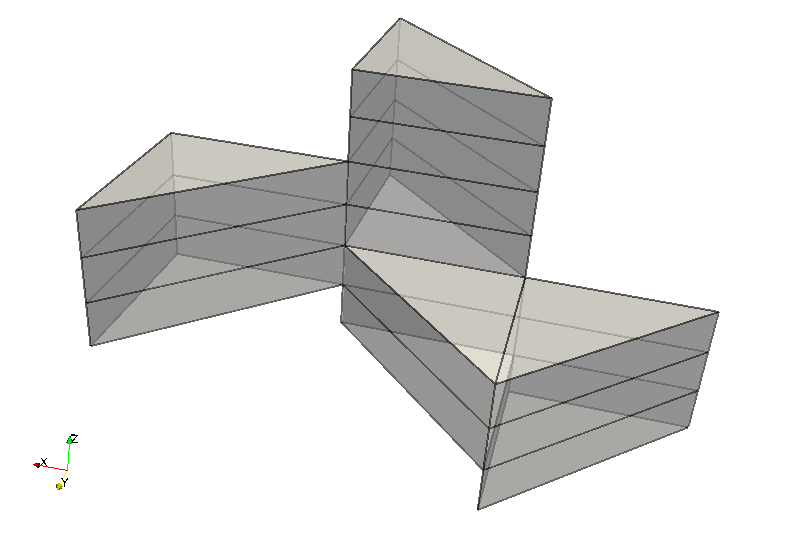
\includegraphics[height=0.5\textheight]{mesh3d}
      \end{center}
    \end{column}
    \begin{column}{0.4\textwidth}
\begin{minted}[fontsize=\tiny]{python}
mesh2d = Mesh(...)
mesh = ExtrudedMesh(mesh2d, [[0, 3],
                             [1, 2],
                             [2, 3],
                             [3, 4]],
                    layer_height=0.25)
\end{minted}
    \end{column}
  \end{columns}
\end{frame}
\begin{frame}[fragile]
  \frametitle{Datatype extension}
  Iteration sets need \emph{four} values per entry.

  \begin{overlayarea}{\textwidth}{0.7\textheight}
    \begin{onlyenv}<1>
      \begin{itemize}
      \item \textbf{allocation} First two entries control allocation of dofs.

        When assigning dofs to base mesh entities, we must consider
        full column.
      \item \textbf{iteration} Second two control iteration.

        When iterating over entities, we can't iterate over ``exposed''
        interior facets.

      \item Need to attach these to \emph{all} base mesh entities.
      \end{itemize}
    \end{onlyenv}
    \begin{onlyenv}<2>
      \begin{columns}
        \begin{column}{0.6\textwidth}
          \begin{center}
            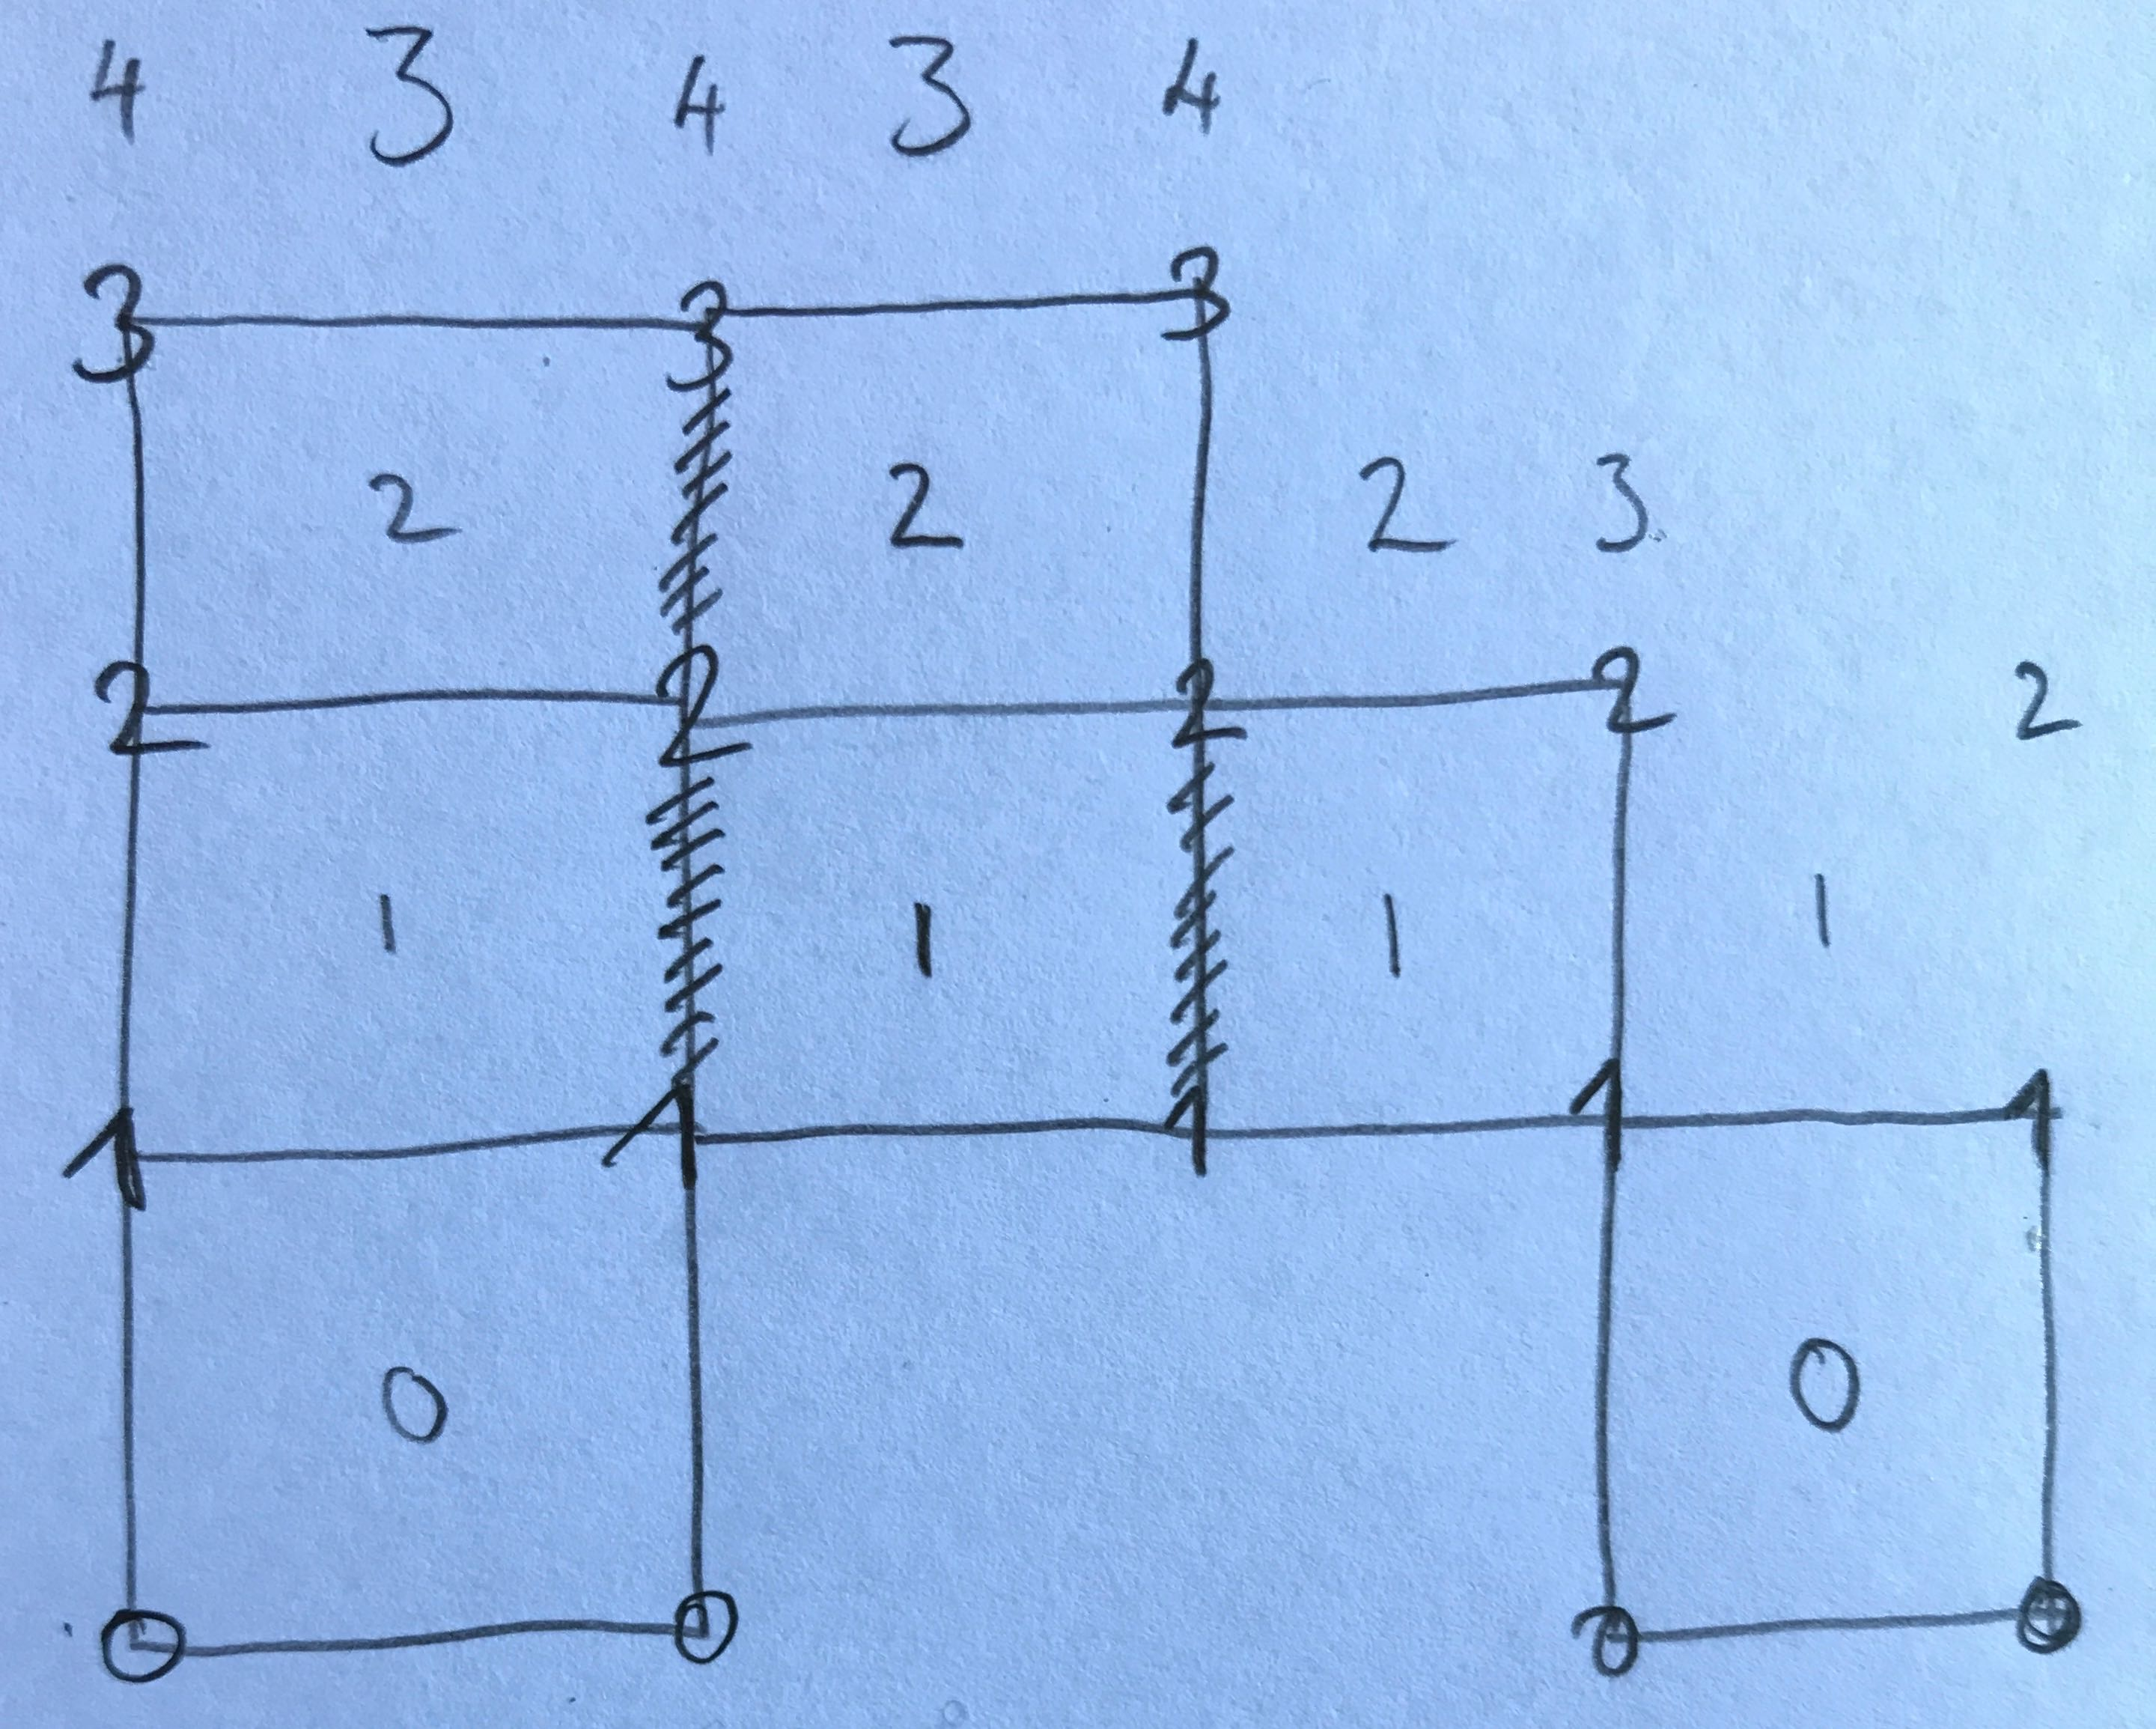
\includegraphics[width=\textwidth]{topology-2d-facets}
          \end{center}
        \end{column}
        \begin{column}{0.5\textwidth}
\begin{minted}[fontsize=\tiny]{python}
interior_facets = ExtrudedSet(2,
                   layers=[[0, 3, 1, 3],
                           [1, 3, 1, 2]])
\end{minted}
        \end{column}
      \end{columns}
    \end{onlyenv}
  \end{overlayarea}
\end{frame}

\begin{frame}[fragile]
  \frametitle{Kernel extension}
  \begin{itemize}
  \item GungHo \emph{kernel} contains iteration over layers
  \item So now we need to provide this information at runtime
  \item Just a directly accessed data array
  \item This needs to be part of kernel API
  \end{itemize}
  \begin{columns}
    \begin{column}{0.5\textwidth}
\begin{minted}[fontsize=\tiny]{fortran}
subroutine old(A, B, nlayers)
   ...
   integer, intent(in) :: nlayers

   do k = 0, nlayers-1
    ...
   end do
end subroutine old
\end{minted}
    \end{column}
    \begin{column}{0.5\textwidth}
\begin{minted}[fontsize=\tiny]{fortran}
subroutine new(A, B, lstart, lend)
   ...
   integer, intent(in) :: lstart, lend

   do k = lstart, lend-1
    ...
   end do
end subroutine new
\end{minted}
    \end{column}
  \end{columns}
\end{frame}

\begin{frame}
  \frametitle{Boundary conditions}
  \begin{itemize}
  \item As ever, strong conditions are painful
  \item It is no longer the case that only nodes on the bottom/top
    cell are killed
  \item I maintain a bitmask on each cell that marks which topological
    entities on the cell are exposed
  \item Then when assembling I can determine which dofs to drop on the
    floor
  \item This is easier if you never build sparse matrices: what's the
    status here?
  \end{itemize}
\end{frame}

\begin{frame}
  \frametitle{Firedrake support}
  \begin{itemize}
  \item Support is still WIP (interior facets)
  \item We squash interior facets geometrically, but not
    topologically.
  \item Then we never iterate over these facets.
  \item They could be left exposed, but now need new iteration type.
  \item An alternate option would be mixed cell shape (ugh!)
  \end{itemize}
\end{frame}
\end{document}
